%!TEX TS-program = xelatex
\documentclass[]{friggeri-cv}
\usepackage{afterpage}
\usepackage{hyperref}
\usepackage{color}
\usepackage{xcolor}
\usepackage{smartdiagram}
\usepackage{fontspec}
% if you want to add fontawesome package
% you need to compile the tex file with LuaLaTeX
% References:
%   http://texdoc.net/texmf-dist/doc/latex/fontawesome/fontawesome.pdf
%   https://www.ctan.org/tex-archive/fonts/fontawesome?lang=en
%\usepackage{fontawesome}
\usepackage{metalogo}
\usepackage{dtklogos}
\usepackage[utf8]{inputenc}
\usepackage{tikz}
\usetikzlibrary{mindmap,shadows}
\hypersetup{
    pdftitle={},
    pdfauthor={},
    pdfsubject={},
    pdfkeywords={},
    colorlinks=false,           % no lik border color
    allbordercolors=white       % white border color for all
}
\smartdiagramset{
    bubble center node font = \footnotesize,
    bubble node font = \footnotesize,
    % specifies the minimum size of the bubble center node
    bubble center node size = 0.5cm,
    %  specifies the minimum size of the bubbles
    bubble node size = 0.5cm,
    % specifies which is the distance among the bubble center node and the other bubbles
    distance center/other bubbles = 0.3cm,
    % sets the distance from the text to the border of the bubble center node
    distance text center bubble = 0.5cm,
    % set center bubble color
    bubble center node color = pblue,
    % define the list of colors usable in the diagram
    set color list = {lightgray, materialcyan, orange, green, materialorange, materialteal, materialamber, materialindigo, materialgreen, materiallime},
    % sets the opacity at which the bubbles are shown
    bubble fill opacity = 0.6,
    % sets the opacity at which the bubble text is shown
    bubble text opacity = 0.5,
}

\addbibresource{bibliography.bib}
\RequirePackage{xcolor}
\definecolor{pblue}{HTML}{0395DE}

\begin{document}
\header{Mulyahadi}{Jatikusuma}
      {Computer Scientist}
      
% Fake text to add separator      
\fcolorbox{white}{gray}{\parbox{\dimexpr\textwidth-2\fboxsep-2\fboxrule}{%
.....
}}

% In the aside, each new line forces a line break
\begin{aside}
  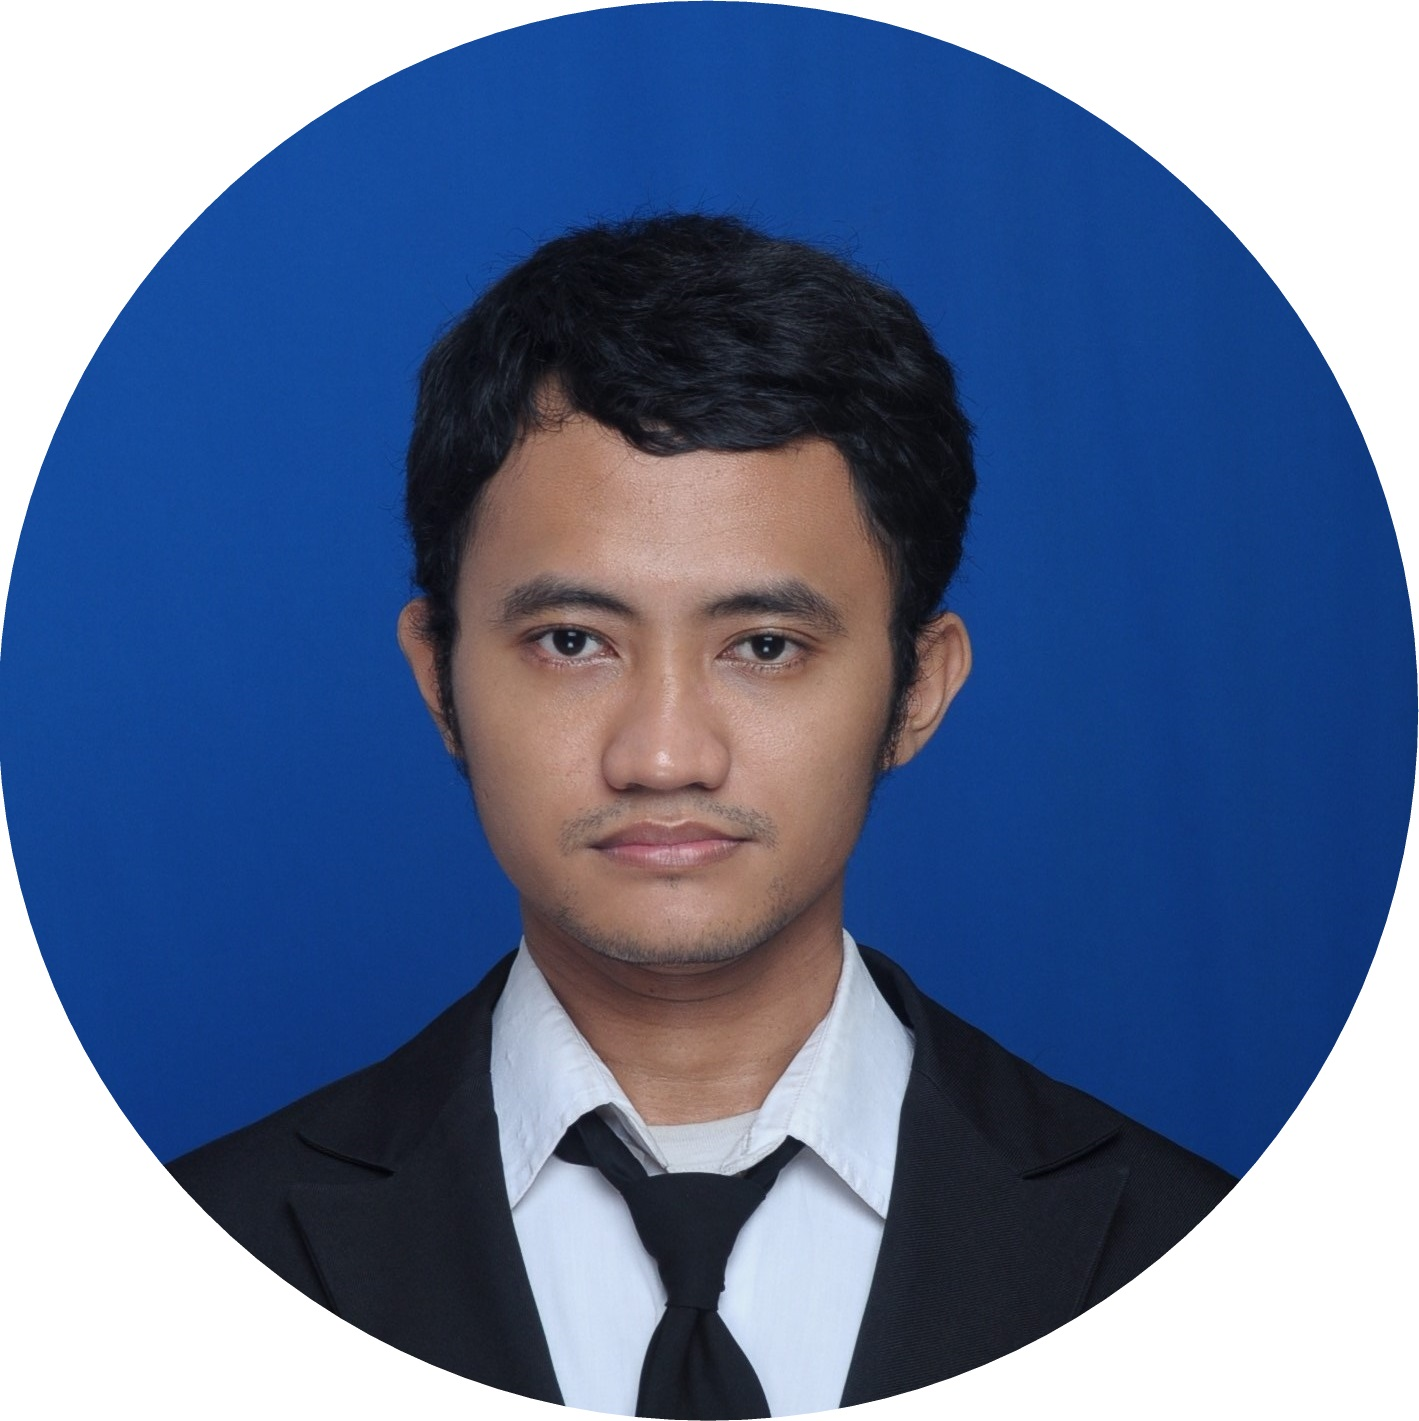
\includegraphics[scale=0.1]{img/mul_circle.jpg}
  \section{Address}
	Jalan Kaliurang Km 4.5  
	Perumahan Swakarya No. 26
    Sleman, Yogyakarta
    ~
  \section{WA \& Facebook}
    +628567641979
    \href{https://www.facebook.com/mulyahadi.j}{Mulyahadi}
    ~
  \section{Mail}
    \href{mailto:mhaidjgm@gmail.com}{\textbf{mhadijgm@}\\gmail.com}
    ~
  \section{Git}
    \href{https://github.com/auaheuyap}{github.com/auaheuyap}
    ~
  % use  \hspace{} or \vspace{} to change bubble size, if needed
  \section{Programming}
    \smartdiagram[bubble diagram]{
        \textbf{C++},
        \textbf{Java},
        \textbf{Open}\\\textbf{GL},
        \textbf{VTK},
        \textbf{Postgre}\\\textbf{SQL},
        \textbf{Perl},
        \textbf{HTML}\\\textbf{/CSS},
        \textbf{PHP},
        \textbf{Tex}
    }
    ~
  \section{Personal Skills}
    \smartdiagram[bubble diagram]{
        \textbf{Team}\\\textbf{Player},
        \textbf{Initiative},
        \textbf{Curiosity},
        \textbf{Problem}\\\textbf{Solving},
        \textbf{\vspace{2mm}Manage\vspace{2mm}},
        \textbf{Organize}
    }
    ~
\end{aside}
~
\section{Project}
\begin{entrylist}
  \entry
    {}
    {Simulasi Fluida Dinamis}
    {}
    {Simulasi fluida untuk memodelkan sistem \textit{rip current} berdasarkan model \textit{Smoothed Particle Hydrodynamic} aplikasi DualSPHysics.\\}
  \entry
    {}
    {Quaternion untuk Sistem Kamera Virtual}
    {}
    {Mengimplementasikan quaternion untuk sistem kamera virtual 3D \textit{tracking} dan interaktif menggunakan OpenGL.\\}
  \entry
   {}
   {Pembuatan \textit{Mesh} dari Kumpulan Titik}
   {}
   {Membuat \textit{mesh} dari sekumpulan titik kordinat menggunakan library Triangulasi Delaunay 3D, API Grafis Visual Tool Kit.\\}
  \entry
    {}
    {Sistem Informasi Tiket Bioskop}
    {}
    {Mengimplementasikan konsep OOP C++ menjadi sistem informasi pemesanan tiket bioskop.\\}
  \entry
    {}
    {Sistem Informasi Katering Online}
    {}
    {Mengimplementasikan konsep OOP Java menjadi sistem informasi katering online.\\}
  \entry
	{}
	{\textit{Model Checking} Semaphore dan Protokol Syzmanski}
	{}
	{Verifikasi dan validasi algoritma Semaphore dan protokol Syzmanski untuk \textit{mutual exclusiveness} menggunakan Promela SPIN.\\}
  \entry
	{}
	{Lexical Analysis Bahasa Pemrograman Perl}
	{}
	{Memecah kode program bahasa pemrograman Perl ke dalam token-token.\\}
  


\end{entrylist}
\\
\section{Education}
\begin{entrylist}
  \entry
    {2012 - 2017}
    {Bachelor's Degree in Computer Science}
    {Universitas Gadjah Mada}
    {Memiliki konsentrasi Algoritma dan Komputasi, saya tertarik dengan berbagai topik komputasi seperti kriptografi (RNG, \textit{blockchain}), komputasi sains (simulasi fluida), grafika komputer (OpenGL, VTK), verifikasi dan validasi (Promela SPIN), sains manajemen (optimasi), \textit{data mining}, sistem temu balik informasi, \textit{object-oriented programming} dan lain sebagainya.\\}
  \entry  
    {2010 - 2011}
    {Unfinished in Mechanical Engineering}
    {Universitas Indonesia}
    {\\}
  \entry
    {2007 - 2010}
    {High School's Graduate}
    {SMAN 28 Jakarta}
    {\\}
\end{entrylist}

\newpage

\begin{aside}
~
~
~
  \section{OS Preference}
	\textbf{Windows}
\includegraphics[scale=0.40]{img/5stars.png}
    \textbf{GNU/Linux}
\includegraphics[scale=0.40]{img/3stars.png}
    ~
  \section{Places Lived}
    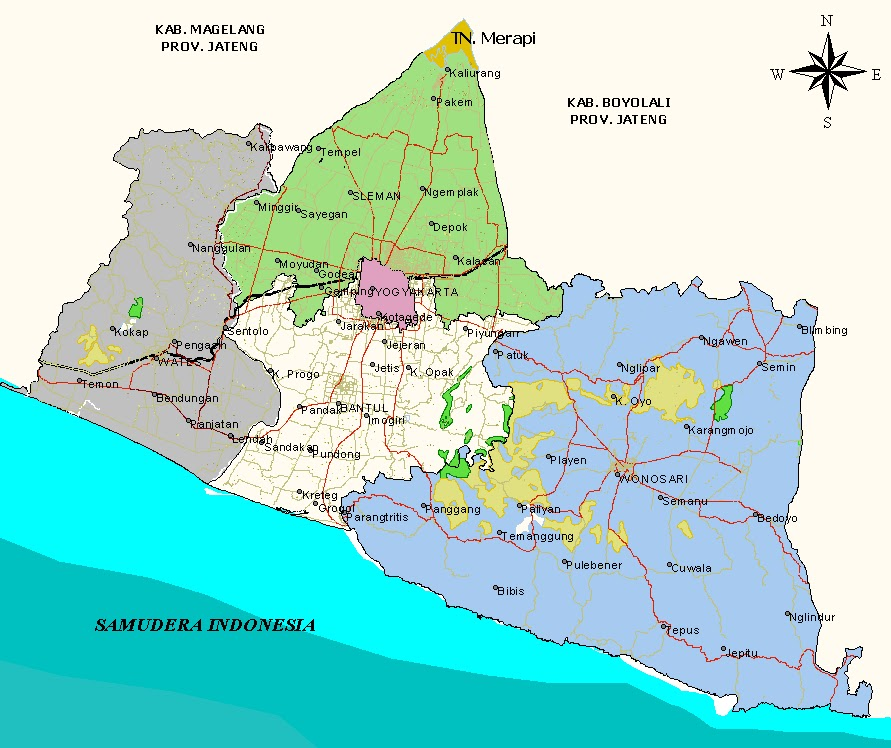
\includegraphics[scale=0.1]{img/peta_diy.jpg}
    ~
  \section{Languages}
    \textbf{Indonesia}
\includegraphics[scale=0.40]{img/5stars.png}
    \textbf{English}
\includegraphics[scale=0.40]{img/5stars.png}
    ~
\end{aside}

\section{Publications}
Jatikusuma, Mulyahadi\\
\textbf{Simulasi dan Validasi Metode Smoothed Particle Hydrodynamic untuk Model Hidrodinamika Rip Current}\\
\emph{Simulation and Validation of Smoothed Particle Hydrodynamic Method for Hydrodynamical Model of Rip Current}
\\

\section{Honors \& Awards}
\begin{entrylist}
  \entry
    {10/2014}
    {Finalis Competetive Programming}
    {C-Compiler}
    {\\}
  \entry
    {10/2015}
    {Finalis Competetive Programming}
    {C-Compiler}
    {\\}
  \entry
    {12/2015}
    {Lulusan terbaik Sertifikasi MTCNA Mikrotik}
    {Mikrotik}
    {\\}
  \entry
	{11/2016}
    {Lulusan terbaik Toefl Test Preparation PPB UGM}
    {TOEFL}
  {\\}
\end{entrylist}

\section{Certifications}
\begin{entrylist}
  \entry
    {12/2015}
    {MTCNA Certificate}
    {Mikrotik RouterOS Training}
    {Skor 83/100}
  \entry
    {11/2016}
    {TOEFL ITP}
    {TOEFL}
    {Skor 587/677}
  \entry
	{3/2015}
	{Workshop Teknologi Berbasis Komputasi Paralel}
	{Lab Komputasi UGM}
	{Workshop big data menggunakan Hadoop}
  \entry
    {10/2016}
    {Omah TI Learning Center 3D Design}
    {Omah TI UGM}
    {Pelatihan IT desain 3D menggunakan Blender}
  \entry
    {10/2016}
    {Omah TI Learning Center Web Application}
    {Omah TI UGM}
    {Pelatihan IT aplikasi web menggunakan Laravel}
\end{entrylist}

%\section{Personal Info}
%\\
%\emph{Saya adalah \textit{fresh graduate} S1 Ilmu Komputer UGM. }
%\\
\begin{flushleft}
\emph{May 27th, 2017}
\end{flushleft}
\begin{flushright}
\emph{Mulyahadi Jatikusuma}
\end{flushright}

\end{document}
